% !TEX root = ../main.tex
%
\chapter{Related Work}
\label{sec:related}

\section{Nerfstudio}
\label{sec:related:nerfstudio}

Nerfstudio \cite{tancik_nerfstudio_2023} represents a significant advancement in making Neural Radiance Fields accessible to non-technical users.
Its design focuses on modularity, ease of use, and integration capabilities, which are crucial for practical applications and academic research.

\paragraph{Modularity}
Nerfstudio is built on a modular framework that allows users to easily customize and extend their NeRF implementations.
This modularity supports various input data formats, making it versatile for different real-world scenarios.
A wide range of existing methods are already well integrated into Nerfstudio, including Instant-GPT \cite{muller_instant_2022}, their own Nerfacto \cite{noauthor_nerfacto_nodate} method that combines various existing techniques, and several of the above mentioned extensions \cite{haque_instruct-nerf2nerf_2023,jan-niklas_dihlmann_signerf_2024}.

\paragraph{Real-Time Web Viewer}
One of the standout features of Nerfstudio is its real-time web viewer, which enables visualization of NeRF training and outputs directly through a web browser.
This eliminates the need for high-end local GPU setups, broadening the tool's accessibility \cite{noauthor_nerfstudio-projectviser_2024}.

\begin{figure}[h!]
  \centering
  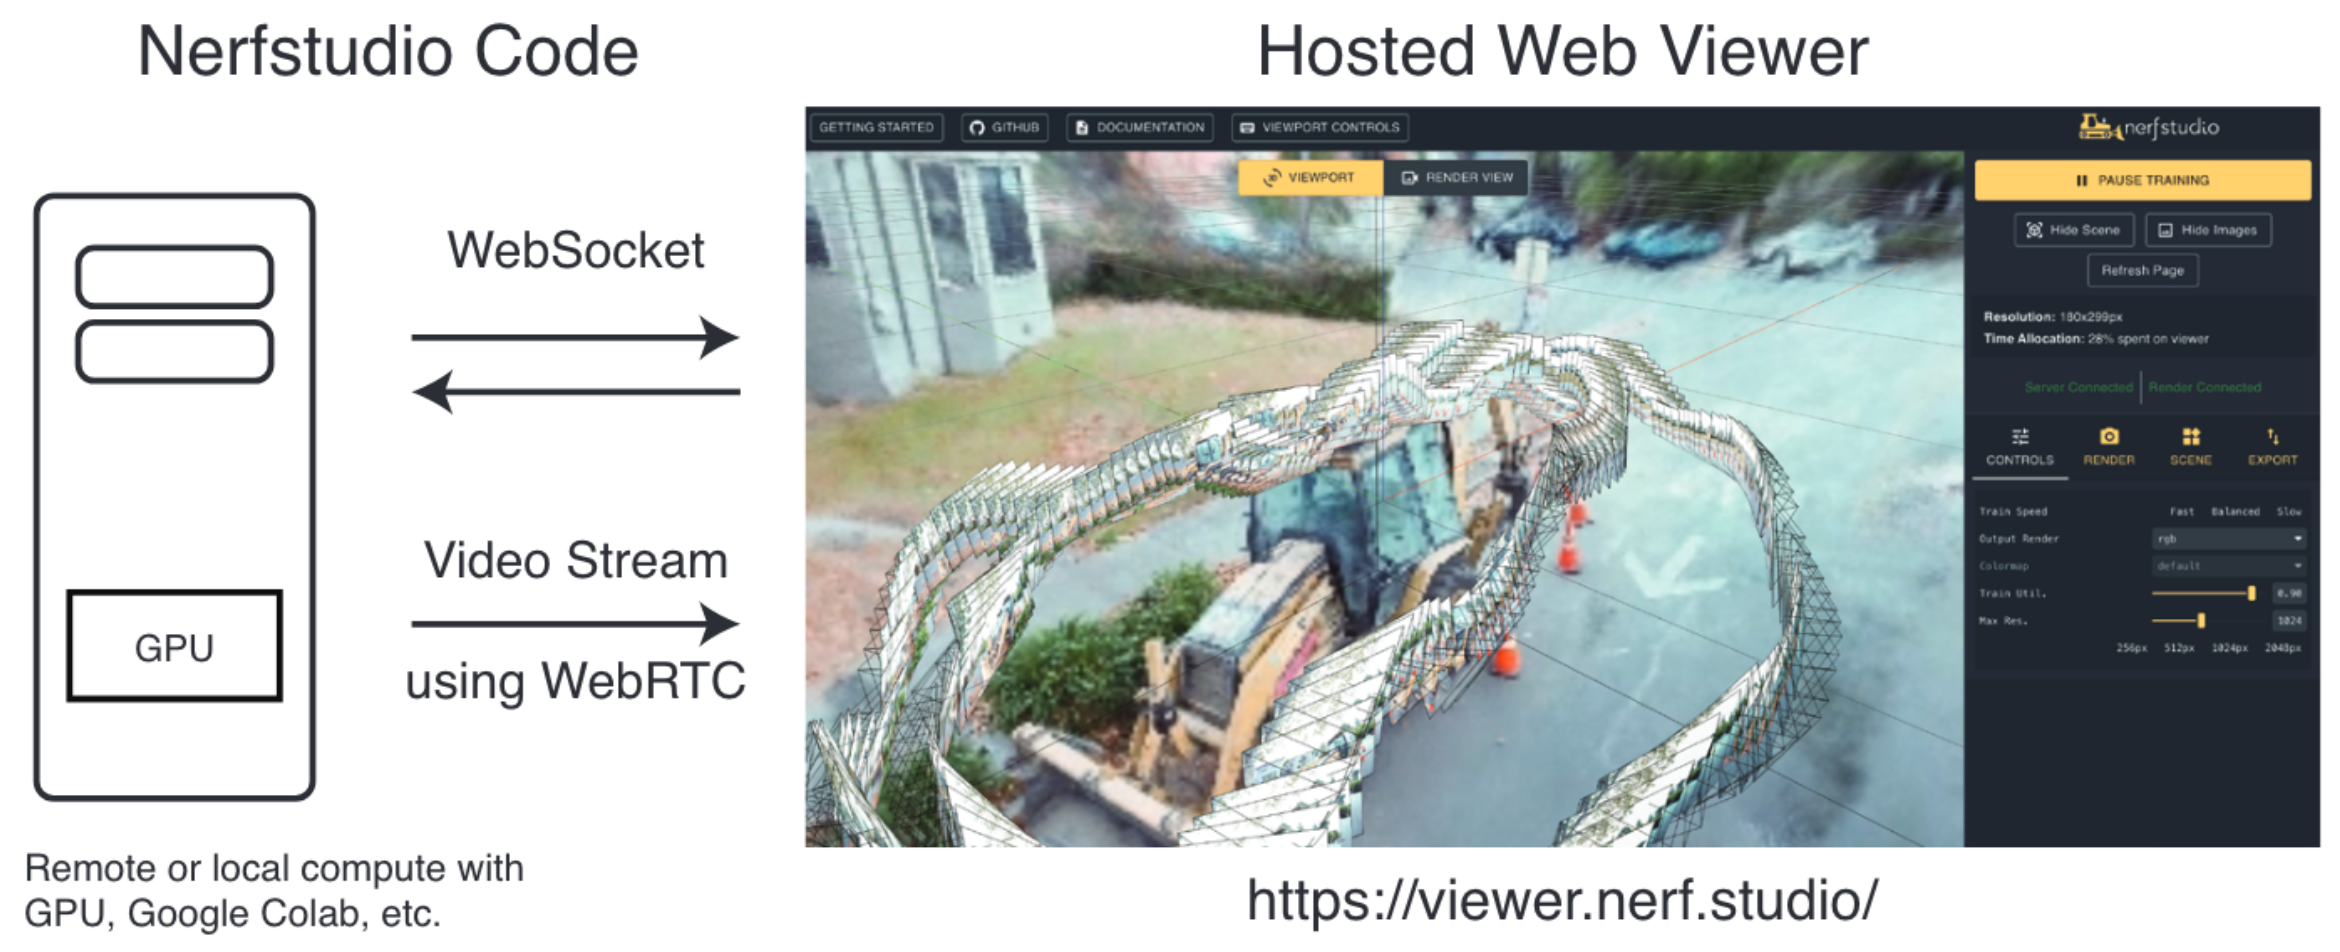
\includegraphics[width=0.7\textwidth]{figures/related-nerfstudio-viewer.png}
  \caption{Nerfstudio's real-time web viewer. (from \cite{tancik_nerfstudio_2023})}
  \label{fig:nerfstudio-viewer}
\end{figure}

\paragraph{Flexibility of Data Handling}
Nerfstudio simplifies the process of importing and exporting data, supporting a wide range of formats to support a variety of use-cases.
Users can easily import images and videos, including data from mobile capture apps such as Polycam \cite{noauthor_polycam_nodate} and Record3D \cite{noauthor_record3d_nodate}.
Additionally, the framework supports exporting results in various formats such as videos, point clouds, and meshes.
This flexibility allows users to integrate NeRF outputs into diverse creative and technical applications.

\paragraph{Community and Open-Source Contribution}
Being open-source, Nerfstudio encourages community-driven development and continuous improvement, facilitating updates that keep pace with the latest research and technological advances.
This openness also allows users to adapt the tool to their specific needs.

\paragraph{Limitiations}

Despite advancements, Nerfstudio's technical complexity and reliance on command-line interfaces for key operations like model training and data preprocessing remain significant barriers.
These aspects limit its accessibility to those with specific technical skills and deter broader creative uses.
The user experience still requires technical knowledge, underscoring the need for more intuitive interfaces that simplify interaction and expand its user base beyond technical specialists.

\section{Luma AI}
\label{sec:related:lmua}

Luma AI \cite{ai_luma_nodate} is making Neural Radiance Fields accessible to non-technical users in a commercial space.
This platform leverages augmented reality (AR) to guide users through the capture process, greatly simplifying the creation of NeRFs from everyday smartphones.

\paragraph{Guided Capture Process}
Luma AI utilizes AR to assist users in capturing images from optimal angles and distances, ensuring that the collected data is suitable for NeRF generation.
This guided process reduces the complexities involved in capturing the necessary footage for effective NeRF modeling.

\paragraph{Cloud-Based NeRF Generation}
Once the footage is captured, it is automatically processed in Luma AI’s cloud-based system to generate a NeRF, requiring no user input for configuration.
This automation not only simplifies the user experience but also makes powerful 3D reconstruction technology readily accessible to a broad audience.

\paragraph{Viewing and Editing}
Created scenes can be viewed directly within the app or through a web browser. 
While the editing capabilities are limited, users can make basic adjustments, reshoot parts of the scene, and interact with the generated NeRF in an intuitive manner.
The features here are similar to what is offered in Nerfstudio's viewer \fref{fig:nerfstudio-viewer}, but with a more modern user-interface.

\paragraph{Export Capabilities}
Luma AI offers various export formats for the generated scenes, allowing users to utilize these outputs in different applications or platforms, further enhancing the utility of the captured NeRFs.
They also provide a social platform for sharing and viewing NeRFs, fostering a community around the technology.

\paragraph{Limitations}
Despite its innovative approach, Luma AI's main limitation lies in the lack of user control over the NeRF training process. 
The automated system, while user-friendly, does not allow for adjustments in the training parameters or the refinement of the final model. 
This lack of control can result in less than optimal NeRF outputs for users who may require more precise or customized 3D representations.

